%%%%% Document Setup %%%%%%%%

\documentclass[10pt, twocolumn]{revtex4}    % Font size (10,11 or 12pt) and column number (one or two).

\usepackage{times}                          % Times New Roman font type

\usepackage[a4paper, left=1.85cm, right=1.85cm,
 top=1.85cm, bottom=1.85cm]{geometry}       % Defines paper size and margin length

%\usepackage[font=small,
%labelfont=bf,justification=justified,format=plain]{caption}                      % Defines caption font size as 9pt and caption title bolded


\usepackage{graphics,graphicx,epsfig,ulem}	% Makes sure all graphics works
\usepackage{amsmath} 						% Adds mathematical features for equations

\graphicspath{{Figs/}}

\usepackage{etoolbox}                       % Customise date to preferred format
\makeatletter
\patchcmd{\frontmatter@RRAP@format}{(}{}{}{}
\patchcmd{\frontmatter@RRAP@format}{)}{}{}{}
\renewcommand\Dated@name{}
\makeatother

\usepackage{fancyhdr}
\usepackage{booktabs}
\usepackage{tabularx}

\pagestyle{fancy}                           % Insert header
\renewcommand{\headrulewidth}{0pt}
\lhead{A. Baldacchino}                          % Your name
\rhead{An Investigation of Post-Collision Galactic Bodies} 
% Your report title               

\def\bibsection{\section*{References}}        % Position refernce section correctly

%\setlength{\belowcaptionskip}{-10pt}
%\setlength{\intextsep}{5pt}
\setlength{\textfloatsep}{5pt}

\usepackage{hhline}
\usepackage{array}
\usepackage{booktabs}
\renewcommand\tabularxcolumn[1]{m{#1}}
\newcolumntype{Y}{>{\centering\arraybackslash}X}
\newcolumntype{M}[1]{>{\centering\arraybackslash}m{#1}}
\newcolumntype{C}{>{\centering\arraybackslash} m{6cm} }
\usepackage{gensymb}
%\captionsetup[figure]{justification=justified,singlelinecheck=off}


%%%%% Document %%%%%
\begin{document}                     

\title{An Investigation of Post-Collision Galactic Bodies} 
\date{Submitted: 16th March 2018}
\author{A. Baldacchino}
\affiliation{\normalfont L3 Computing, Computing Group C3}

\begin{abstract}              
 
The inevitable collision between the Milky Way (MW) and Andromeda (M31) galaxies is significant to the resulting structure of our local group. We model the collision of the Milky Way and Andromeda as a restricted three body problem in an exploration of how accurately this method can produce real-world results. The galactic cores were modelled as gravitationally softened masses embedded in an NFW potential with the stars simulated as massless test particles. We measured the stellar transfer between galaxies, number density profiles and rotation curves of the post-collision bodies. We found that the more massive core (M31) retained nearly all of its stars  post-collision whereas the MW core retained only $40\%$. $30\%$ of the total initial stars in the system were lost into deep space. We found that our calculated number densities are well fitted by an Einasto profile with fitting parameters for the MW of $\alpha=1.07^{+0.08}_{-0.09}$, $r_{-2}=47^{+3}_{-3}$,  $r_{200}=196^{+1}_{-1}$ and for the M31 body given by $\alpha=0.47^{+0.02}_{-0.03}$, $r_{-2}=32^{+2}_{-1}$,  $r_{200}=237^{+1}_{-1}$. These results show that, using a simplistic model of colliding galaxies and randomised initial conditions, features that are present in the literature can still emerge and be well fit.
\end{abstract}

\maketitle
\thispagestyle{plain} % produces page number for front page

\section{Introduction} 

The Andromeda (M31) and Milky Way (MW) galaxies are the two most massive bodies in our local group and exert considerable influence on its evolution. These galaxies are moving towards each other with a velocity ${\sim}110$ km s\textsuperscript{-1} and so the eventual collision of these bodies will be significant to the future structure and composition of the local group, and also significant to the eventual fate of our own solar system.\textsuperscript{\cite{vanderMarelM31VelocityVector2012}}

Traditionally, simulating the interaction of these two bodies would require an N-body simulation to model the dynamics of the stars, supermassive black holes at the centre of the galaxies, and the dark matter halos surrounding the galaxies. Cox and Loeb (2008) show that this method is viable for predicting the outcome of the collision of the MW and M31 and its reperucssions for our solar system.\textsuperscript{\cite{CoxCollisionMilkyWay2008}}

However, N-body simulations are notoriously computationally expensive. When considering the collision of these galaxies, if we were to model both galaxies with a conservative estimate of the number of stars in these systems, we would require an N-body simulation of $10^{12}$ particles. This is highly impractical due to the computational time that would be required. Therefore, it is worthwhile to explore simplifications that can be made that do not compromise the accuracy of the simulation, and whether such simplified methods can produce realistic post-collision bodies.

A simplification that can be made to this system of colliding galaxies is to model them as a restricted three body problem with the stars modelled as test particles. This has shown to be suitable to investigate stellar configurations by Banik et al (2018).\textsuperscript{\cite{BanikOriginLocalGroup2018}} To further simplify the simulation, the total number of test particles in the system can be reduced to $10^4$. This will provide sufficient particle densities to investigate the resulting formations.

The restricted three body problem is a simplification of the three body problem whereby there is a system of two massive bodies and one or more objects of negligible mass which are modelled as massless test particles. The massive bodies interact only with each other and so their positions can be known analytically. The test particles interact with both massive bodies and so their positions must be determined numerically. As the test particles only interact with the two massive bodies, this significantly reduces computation time. 

Galaxies are known to be embedded in dark matter halos. Therefore, we should consider an alaytical implementation of this in our system of colliding galaxies. Literature from Einasto (1965) and Navarro et al (1996) well document two of the best fitting density profiles for dark matter halos, the Einasto profile and Navarro, Frenk and White (NFW) profile respectively.\textsuperscript{\cite{EinastoConstructionCompositeModel1965}\cite{NavarroStructureColdDark1996}}

Modelling galaxies as point particles can cause them to behave in unphysical ways. Rodionov and Sotnikova (2005) discuss the optimal softening lengths and how this is related to the time step of the simulation.\textsuperscript{\cite{RodionovOptimalChoiceSoftening2005}} They showed that the softening length should be a factor of 1.5-2 times smaller than the mean distance between particles in the densest regions for them to be resolved. They also found that the time step used should be adjusted so that on average a particle should not travel more than $\epsilon/2$ in one time step.

From the literature, we can also learn that a large rotating body of gas collapses into the fundamental plane of rotation through the transfer of momenta in the system with the resulting body forming a disk with stable orbits.\textsuperscript{\cite{EggenEvidencemotionsold1962}}. Once this happens, the body is said to have viralized. In this work, the stars are modelled as test particles so this effect is unable to take place. We will investigate if this has a significant effect on the post-collision structure.
%
%In this work, the MW-M31 system will be modelled using the restricted three body problem, incorporating a dark matter halo and softened gravitational potentials, in an investigation of how viable this method is when considering colliding galaxies.

\section{Method}

In this investigation, the MW and M31 galaxies were modelled as two galactic cores with stars as test particles. The galactic cores are the massive bodies required by the restricted three body problem with masses based upon those found in the literature. The force on each galactic core is equal and opposite and given by Newton's law of gravitation:
\begin{equation}
\pmb{F_{21}} = -\frac{GM_{1}M_{2}}{|\pmb{r_{12}}|^3} \pmb{r_{12}},
\label{force_eq}
\end{equation}
where $\pmb{F_{21}}$ is the force on core two due to core one, $G$ is Newton's universal gravitational constant, $M_{1}$ and $M_{2}$ are the masses of each galactic core and $\pmb{r_{12}}$ is the vector from core one to core two. Hereafter, the MW galactic core is represented by core one and M31 by core two.

The stars have an attractive force component from both galactic cores with their equation of motion given by:
%\begin{multline}
%\frac{d^2\pmb{r}}{dt^2} = G \bigg( \frac{M_{MW}(\pmb{r_{MW}}-\pmb{r})}{|\pmb{r_{MW}}-\pmb{r}|^3} +\\
%\frac{M_{M31}(\pmb{r_{M31}}-\pmb{r})}{|\pmb{r_{M31}}-\pmb{r}|^3} \bigg),
%\label{motion_eq}
%\end{multline}
\begin{equation}
\frac{d^2\pmb{r}}{dt^2} = \sum^2_{i=1}\frac{GM_i(\pmb{r_{i}}-\pmb{r})}{|\pmb{r_{i}}-\pmb{r}|^3}.
\label{motion_eq}
\end{equation}
Here $\pmb{r}$ is the position vector of the star, $\pmb{r_{i}}$ is the position vector of each galactic core and $M_{i}$ are the total masses of each core.

When modelling the galactic cores as point masses they interact with very large deflection angles. In reality, galactic mass is spread over its stellar bulge, disk, and dark matter halo, so it is unrealistic to assume a point like central core. To address this, we introduce a softening length term in the gravitational potential so that it no longer acts like a point mass. Equation (\ref{force_eq}) then becomes\textsuperscript{\cite{C.C.DyerSofteningNbodysimulations1993}}
\begin{equation}
\pmb{F_{21}} = -\frac{ G M_{1} M_{2} } { (|\pmb{r_{12}}|^2+\epsilon^2)^\frac{3}{2}} \pmb{r_{12}},
\label{softened_eq}
\end{equation}
where $\epsilon$ is the softening length term and the other parameters are the same as in equation (\ref{force_eq}). 

To further improve the realism of this simulation, we introduce a dark matter halo for each of the galactic cores. Galactic dark matter halos can be well described by a Nevarro, Frenk and White (NFW) profile.\textsuperscript{\cite{NavarroStructureColdDark1996}} This is a spherically symmetric density profile which can be described by:
\begin{equation}
\rho(r) = \rho_0\left(\frac{r}{r_s}\right)^{-1}\left(1+\frac{r}{r_s}\right)^{-2},
\label{NFWdens_eq}
\end{equation}
where $\rho(r)$ is the dark matter density at radius, $r$, from the centre of the halo, $r_s$ is the scale radius which is a parameter fit to each halo, and $\rho_0$ is defined by:
\begin{equation}
\rho_0 = \frac{200}{3}\frac{c^3}{\ln(1+c)-\frac{c}{1+c}}\rho_{crit},
\label{rho0_eq}
\end{equation}
where $\rho_{crit}$ is the critical density of the universe, $r_{200}$ is known as the virial radius, inside which the mean enclosed density is equal to $200\rho_{crit}$, $c=r_{200}/r_s$ is known as the concentration parameter.\textsuperscript{\cite{ReadLocalDarkMatter2014}} The integral of equation (\ref{NFWdens_eq}) defines the mass enclosed inside radius, $r$, and is given by:
\begin{equation}
M_{enc}(r)=4\pi\rho_0r_s^3\left(-\frac{r}{r_s+r}+\ln\left(1+\frac{r}{r_s}\right)\right).
\label{Menc_eq}
\end{equation}

We now adjust the simulation so that the total mass of each galactic core is defined as $M_{200}$ where $M_{200}=M_{enc}(r_{200})$ which can be calculated from equation (\ref{Menc_eq}) using literature values for $r_s$ and $r_{200}$ for each galaxy.

To study the viability of the restricted three body method for the simulation of colliding galaxies, the stellar transfer between the galaxies, density profiles and rotation curves of the resulting bodies were analysed. The density profiles of each galactic core are calculated by dividing each halo into a set of concentric spherical shells centred on the galactic core. The normalised number density for each bin was then calculated using
\begin{equation}
\frac{n(N_{bin},r_{min},r_{max})}{\langle n\rangle} = \frac{N_{bin}}{N_{tot}}\frac{r_{200}{}^3}{r_{max}{}^3-r_{min}{}^3},
\label{ndensitybin_eq}
\end{equation}
where $n/\langle n\rangle$ is the number density normalised by the mean number density over the entire halo, $N_{bin}$ is the number of stars in the bin, $N_{tot}$ is the total number of stars over all bins, $r_{min}$ and $r_{max}$ are the boundaries of the bin.

Number density profiles in the literature are typically well fitted by either an NFW or an Einasto profile. Firstly, a normalised NFW profile was fitted which is given by:
\begin{equation}
\frac{n(r)}{\langle n\rangle}=\rho(r)\frac{\frac{4}{3}\pi r_{200}{}^3}{M_{enc}(r_{200})}.
\label{normNFW_eq}
\end{equation}

An Einasto profile can also be fitted to our data which introduces an extra free parameter, $\alpha$, compared to the NFW profile and so may be able to better fit our data.\textsuperscript{\cite{EinastoConstructionCompositeModel1965}\cite{NavarroinnerstructureLCDM2004}\cite{Newtontotalsatellitepopulation2017}} The Einasto profile, normalised by the mean number density in the halo, is given by:
\begin{equation}
\frac{n(r)}{\langle n\rangle} = \frac{\alpha r_{200}{}^3 \exp\left(-\frac{2}{\alpha}\left( \frac{r}{r_{-2}} \right)^\alpha\right)}{3r_{-2}{}^3 \left( \frac{\alpha}{2} \right)^{\frac{3}{\alpha}}\gamma \left(\frac{3}{\alpha},\frac{2}{\alpha}\left(\frac{r_{200}}{r_{-2}}\right)^{\alpha}\right)},
\label{normedeinasto_eq}
\end{equation}
where $r_{200},r_{-2},\alpha$ are parameters that are varied to fit the profile to the data set, and $\gamma$ is given by:
\begin{equation}
\gamma(s,x)=\int_0^xt^{s-1}\exp(-t)dt.
\end{equation}

If we assume our post-collision bodies to have virialized, then classically, the tangential velocity of the stars in our post-collision bodies can be related to the mass enclosed, and is given by:
\begin{equation}
v(r) = \left(\frac{GM_{enc}(r)}{r}\right)^{\frac{1}{2}},
\end{equation}
where $r$ is the distance from the centre of the halo and $M_{enc}$ is defined in equation (\ref{Menc_eq}).

\subsection*{Computational Model}

From our preliminary investigation, the SciPy black box integrator\textsuperscript{\cite{scipyintegrateode}} and Runge-Kutta (4th order, RK4)\textsuperscript{\cite{ButcherNumericalmethodsordinary2008}} methods of integration were selected for this computation. The collision of the galaxies was simulated in two parts. Firstly, the galactic core positions and velocities were computed using the SciPy integrator solving equation (\ref{softened_eq}). Each core was modelled with an NFW dark matter halo originating from each core's centre and a softened gravitational potential; the parameters for both the NFW profile and the softened gravitational potential are given in Table \ref{params_tab}. The positions and velocities of the stellar test particles were then computed using the RK4 method solving equation (\ref{motion_eq}). A time step of $2 \times 10^5$ years was used for both the SciPy and RK4 integrations.

The initial separation of the galactic cores was chosen to be 600 kpc. The M31 core was given an initial velocity towards the MW core of $110$ km s\textsuperscript{-1} and a transverse velocity of $10$ km s\textsuperscript{-1}. These parameters were selected as they are consistent with the literature.\textsuperscript{\cite{vanderMarelM31VelocityVector2012}\cite{CoxCollisionMilkyWay2008}} Initially, the stars were uniformly distributed in a disk centred on the core and extending to a maximum stellar distance, $R_{max}$. The stellar disc of M31 was inclined and rotated by $45\degree$ relative to the MW disc so that the galaxies were not colliding as two edge on discs. The stars' velocities were set so that initially they orbited in circular stable orbits around their respective cores. The parameters used for each galaxy are given in Table \ref{params_tab}. The simulation was run for 20 Gyrs, as preliminary testing revealed that this allowed enough time for the galaxies to interact and reform two distinct bodies. 
\begin{table}[h!]
\begin{center}
\begin{tabularx}{0.5\textwidth}{  Y Y Y Y Y  }
\hhline{=====}
& $R_{max}$ (kpc) & $\epsilon$ (kpc)& $r_s$ (kpc)& $r_{200}$ (kpc)\\ \hline
Milky Way & $40$ & $7.5$ & $12.5$ & $200$ \\ 
Andromeda & $67$ & $7.5$ & $34.6$ & $240$ \\ \hline
\end{tabularx}
\caption{A table displaying the parameters used in the simulation. The parameters correspond to the maximum initial stellar radius, $R_{max}$, the softening length term, $\epsilon$, and the fitting parameters for an NFW profile, $r_s$ and $r_{200}$.}
\label{params_tab}
\end{center}
\end{table}

The stellar transfer of each galaxy was analysed by tracking, over the duration of the simulation, how many stars were within each galactic core's $r_{200}$ radius as this was deemed a suitable boundary for the edge of each body. Using this method, some stars were double counted as they were within the $r_{200}$ radius of both cores at times around closest approach.

The number density profile of each core was found by generating $20$ logarithmically spaced bins from $r=0$ to $r=r_{200}$ for each galactic core. The number density in each shell was then calculated using equation (\ref{ndensitybin_eq}) and NFW and Einasto profiles were then fitted using equations (\ref{normNFW_eq}) and (\ref{normedeinasto_eq}).

The rotation curves of each galaxy were analysed by initially projecting the positions and velocities of the stars onto a plane. A slit of width $4$ kpc was aligned along the largest velocity gradient and the tangential velocity of the stars were then calculated. As the rotation curves on opposite sides of the galactic core are asymmetric, they were averaged to find the global rotation curve. 

\section{Preliminary Investigation}

In this investigation, a numerical integrator had to be selected to compute the positions of the galactic cores and stars. The accuracy of the Taylor\textsuperscript{\cite{ButcherNumericalmethodsordinary2008}}, RK4\textsuperscript{\cite{ButcherNumericalmethodsordinary2008}} and SciPy black box\textsuperscript{\cite{scipyintegrateode}} numerical integrators were tested using a star orbiting a single galactic core. The solution to this is analytically known, with a fixed radius of $R_0$, allowing for a direct comparison with the numerical results to be made. The time step used in this preliminary investigation was $2 \times 10^5$, which is the same as the time step used in the collision simulation.

\begin{figure}[t!]
\centering
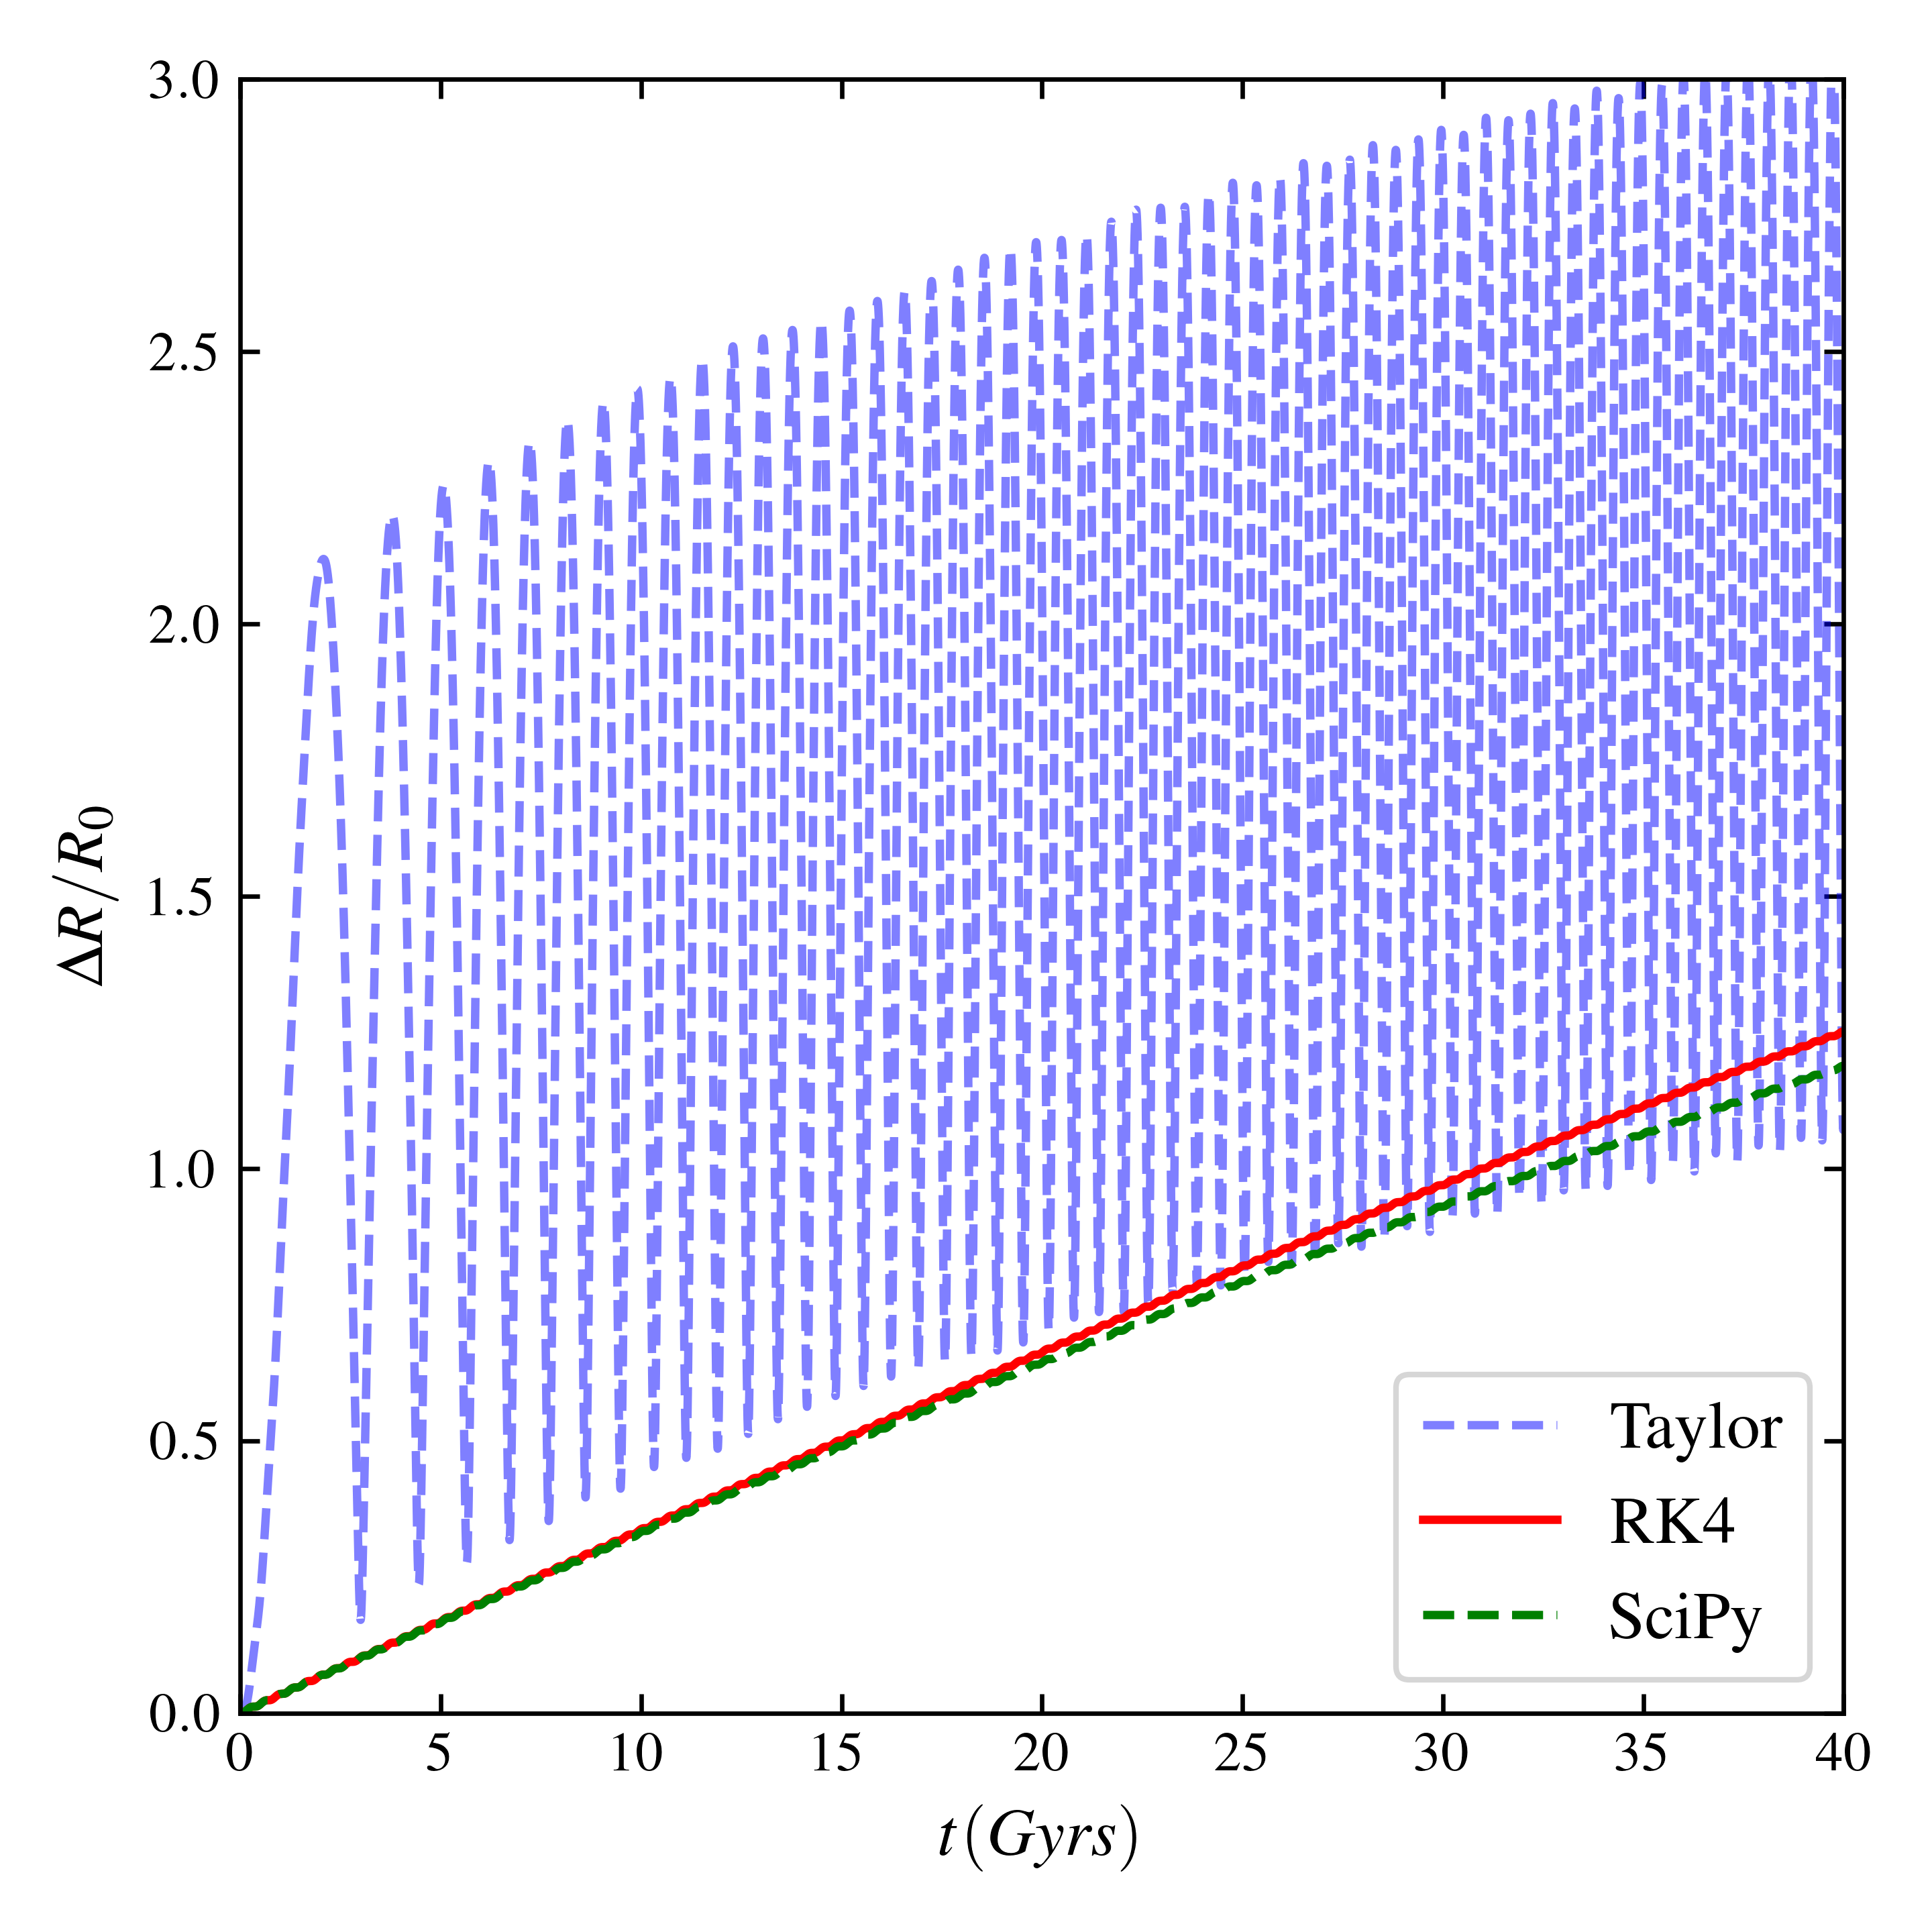
\includegraphics[width=0.5\textwidth]{20180316_122555_INTEGRATOR_ANALYSIS}
\caption{A comparison of the accuracy of the Taylor, Runge Kutta and SciPy black box integrators. This figure shows the variation of the calculated radius of the orbit from the known analytical solution, $R_0$.}
\label{fig: integrator comp}
\end{figure}

We show the results of the comparison of the three integrators in Figure \ref{fig: integrator comp}. This shows that the Taylor method produces a very chaotic result compared to the SciPy and RK4 method. The SciPy and RK4 method are more accurate but still diverge away from the analytical result, reaching $\Delta R/R_{0} \approx 1$ after 40 Gyrs of simulation. These results demonstrate that the Taylor method is inadequate for accurate numerical computation and motivate our use of the RK4 and SciPy black box integrator in this investigation.

\begin{figure}[t!]
\centering
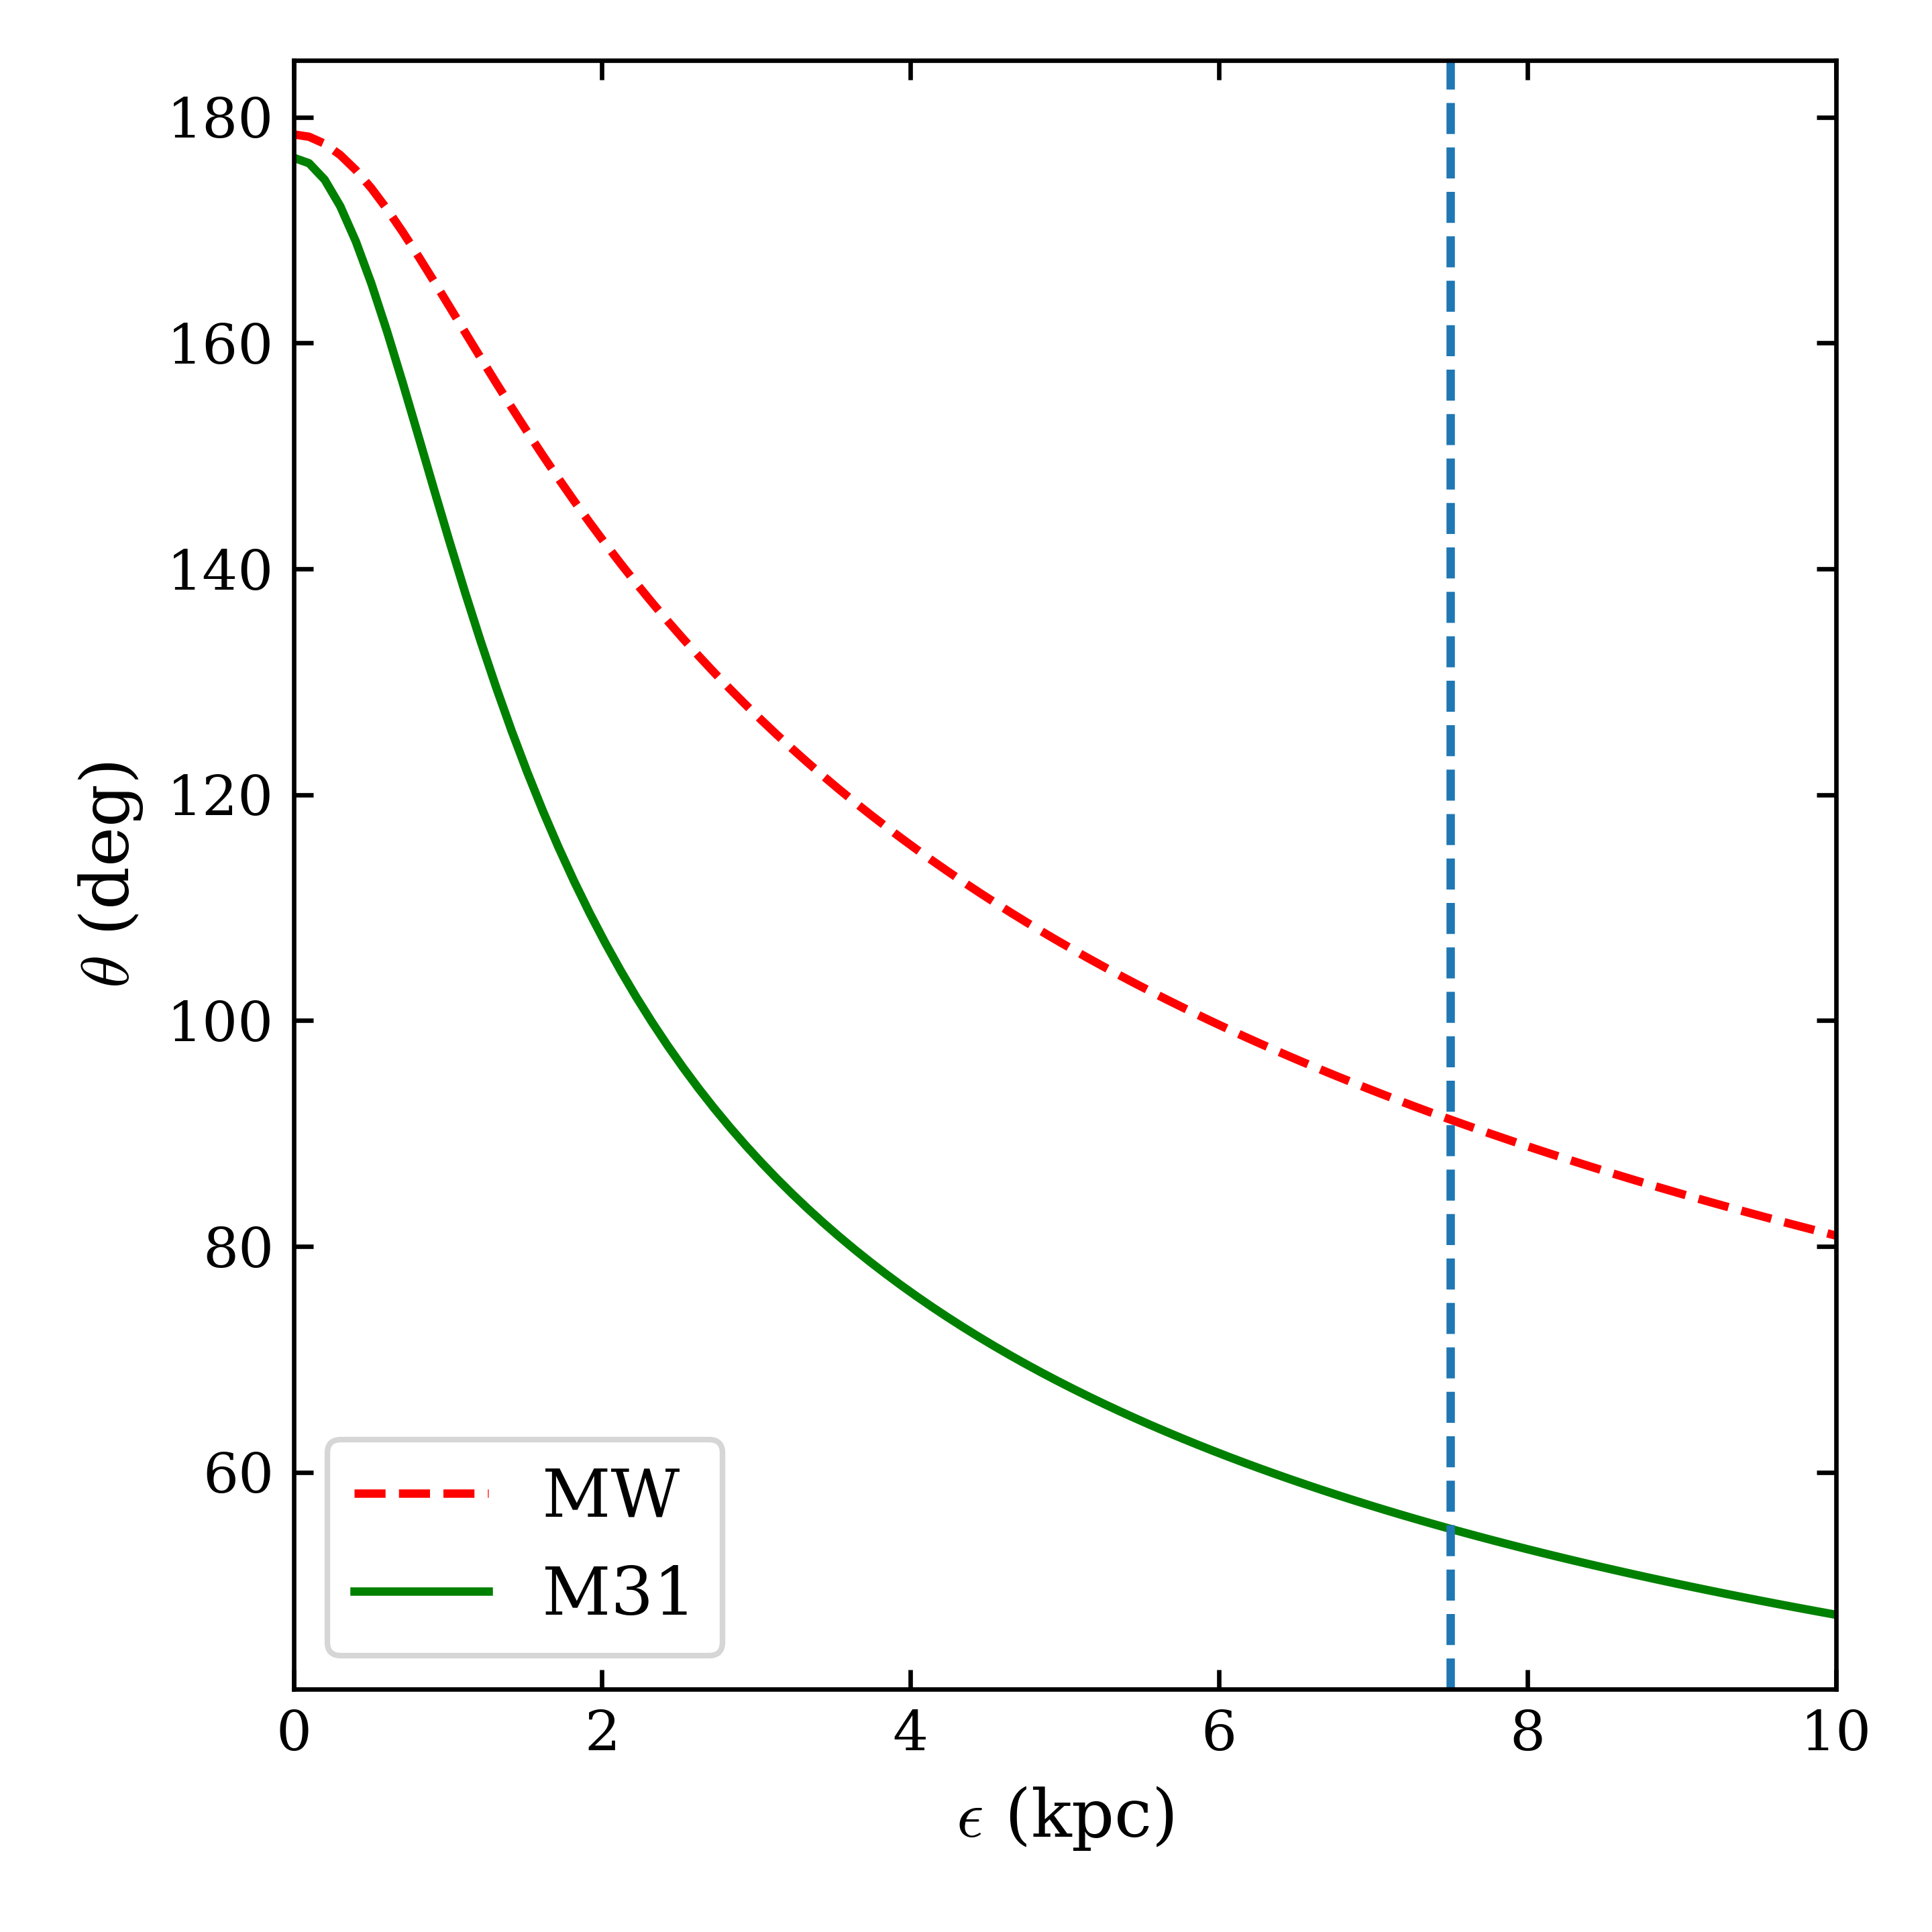
\includegraphics[width=0.5\textwidth]{20180315_010154_SOFTENING_DEFLECTION__5_Gyrs}
\caption{An investigation of how softening length, $\epsilon$, affects the deflection angle, $\theta$, of both galaxies. A vertical line at $\epsilon = 7.5$ kpc is also displayed.}
\label{fig: softening length comparison}
\end{figure}

To determine the optimal value for the softening length, $\epsilon$, we simulated solely the galactic cores (with no test particles) colliding in two dimensions, for a range of $\epsilon$ from $0$ to $10$ kpc with the deflection angle for each galaxy being measured. The deflection angle was defined as the angle between its initial velocity vector and its final  velocity vector whereby a greater value of $\epsilon$ decreased the deflection angle. The result of this investigation is shown in Figure \ref{fig: softening length comparison}. This was performed to find an appropriate value for the softening length that would allow a more real-world like interaction of the galaxies, without significantly artificially affecting the interaction by selecting a softening length value that was too large.  A softening length of $\epsilon=7.5$ kpc was selected for both galaxies as this provided a deflection angle more appropriate for galaxies whilst not losing  resolution in the inner sections of the galaxy for $r<12.5$ kpc which is the value of $r_s$ used for the NFW dark matter halo for the MW core. There were also diminishing returns for increasing $\epsilon$ far beyond $7.5$ kpc.
 
\section{Results} 

The results of the analysis of the post-collision bodies are shown below. Figure \ref{fig: n with r200} shows the evolution of the stellar complement of each core during the collision. The number of stars, $N_{200}$, associated with each core is defined as the number of stars within each bodies $r_{200}$ radius. $N_{initial}$ is the number of stars each body was generated with at the start of the simulation.

\begin{figure}[h!]
\centering
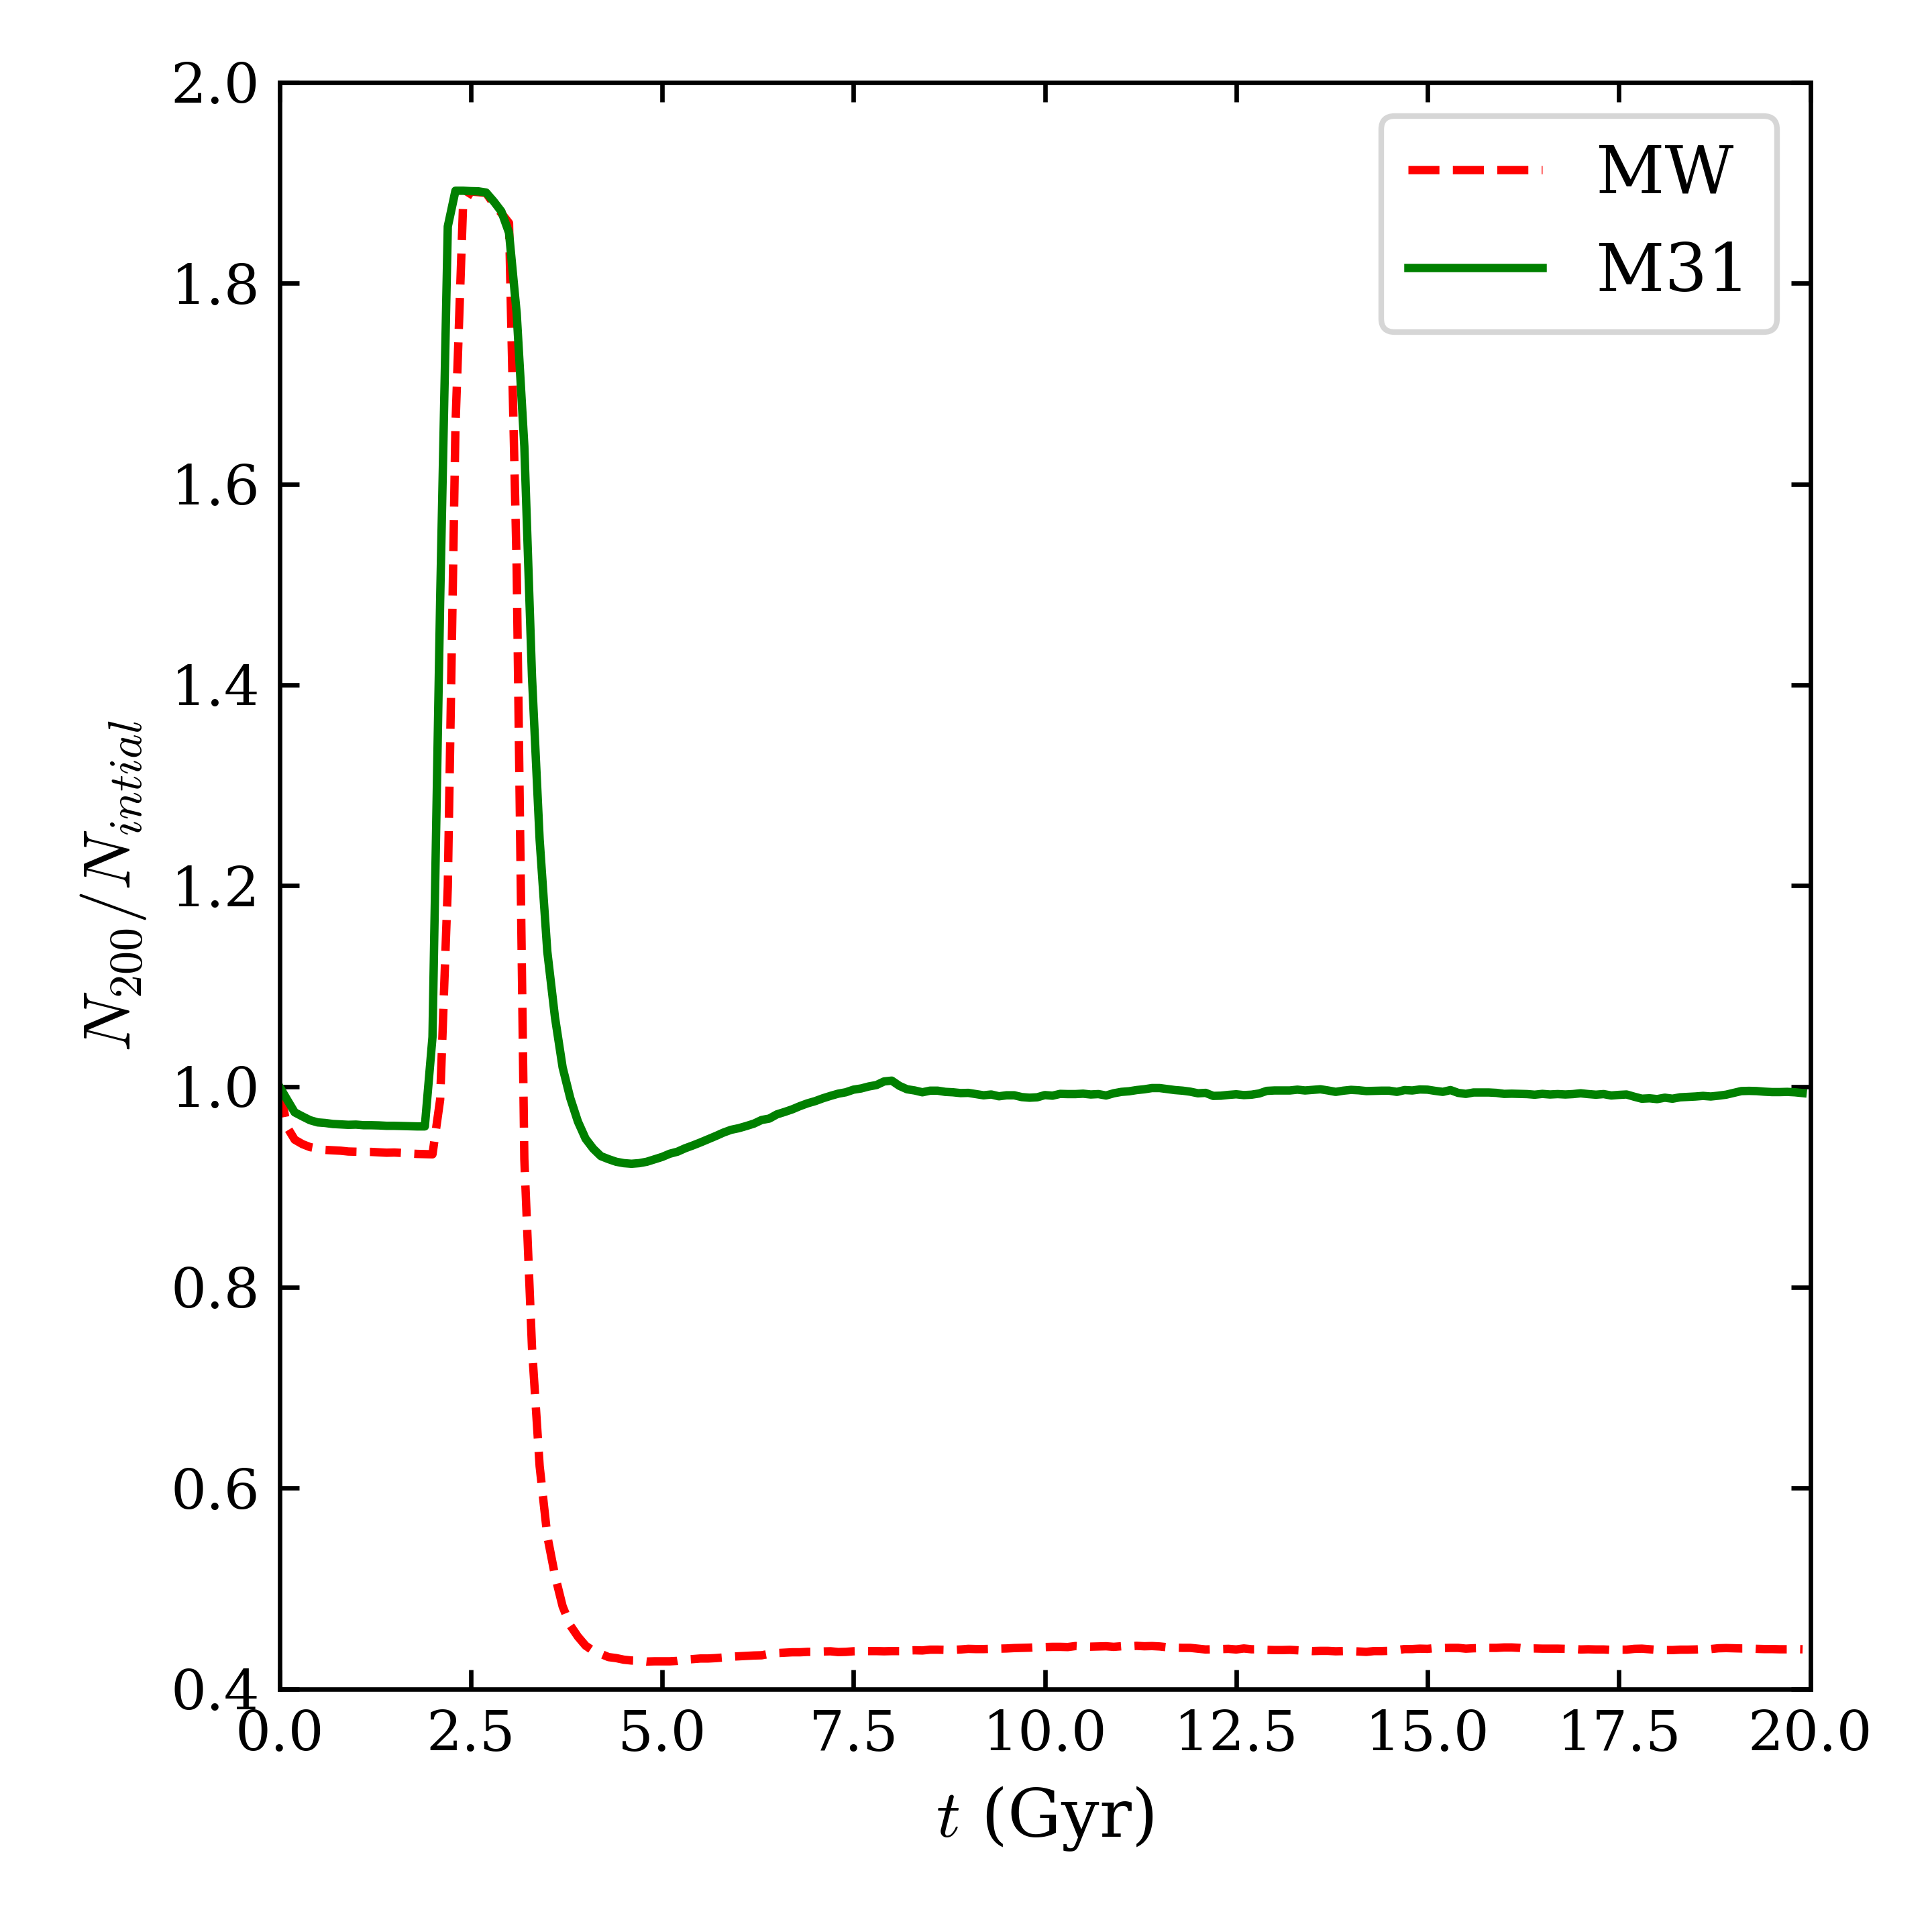
\includegraphics[width=0.5\textwidth]{20180315_005630_N_IN_200_FIG_20_Gyrs}
\caption{The ratio of the number of stars within the $r_{200}$ radius to their initial star count for the MW and M31 cores. Each galaxy has $N_{initial}=5000$ stars.}
\label{fig: n with r200}
\end{figure}
Figure \ref{fig: n with r200} shows that as time progresses, there is a peak as expected in $N_{200}/N_{initial}$ around $t=2.5$ Gyr, the time of closest approach. There is a drop in $N_{200}/N_{initial}$ once the galaxies separate again with the ratio levelling off as the galaxies reform two distinct bodies and are no longer losing stars. The more massive galaxy, M31, retains a similar number of stars post-collision as it had prior to the collision with $N_{200}/N_{initial} \approx 1$ at $t=20$ Gyrs. The MW galaxy, which has a mass ${\sim}0.5$ times that of M31, loses significantly more matter, retaining only $40\%$ of its initial complement at $t=20$~Gyrs due to its lower gravitational pull. As the galaxies can only account for $70\%$ of the total initial star population, this implies that $30\%$ of the stars are lost to deep space due to the collision. In this investigation we define deep space as outside of either core's $r_{200}$ radius.

\begin{table}[h!]
\centering
\begin{tabularx}{0.5\textwidth}{ Y Y Y Y Y }
\hhline{=====}
\multicolumn{5}{c}{NFW} \\ \hline
& $r_s$ (kpc) & $r_{200}$ (kpc) & & $\chi^2_{min}$ \\[3pt] 
MW & $48^{+8}_{-6}$ & $177^{+2}_{-2}$& & $18.17$ \\[3pt] 
M31 & $20^{+1}_{-1}$ & $233^{+1}_{-1}$& & $9.97$\\[3pt] \hhline{=====}
\multicolumn{5}{c}{Einasto} \\ \hline
&  $r_{-2}$ (kpc) & $r_{200}$ (kpc) & $\alpha$ & $\chi^2_{min}$ \\[3pt] 
MW & $47^{+3}_{-3}$ & $196^{+1}_{-1}$ & $1.07^{+0.08}_{-0.09}$ & $0.66$ \\[3pt]
M31 & $32^{+2}_{-1}$ & $237^{+1}_{-1}$ & $0.47^{+0.02}_{-0.03}$ & $1.38$ \\[3pt] \hline
\end{tabularx}
\caption{The parameters that were used to fit NFW and Einasto profiles to the data in Figure \ref{fig: n density MW}. $\chi^2_{min}$ values were calculated using 3$\sigma$ errors.}
\label{table: NFW/Ein params}
\end{table}

\begin{figure}[h!]
\centering
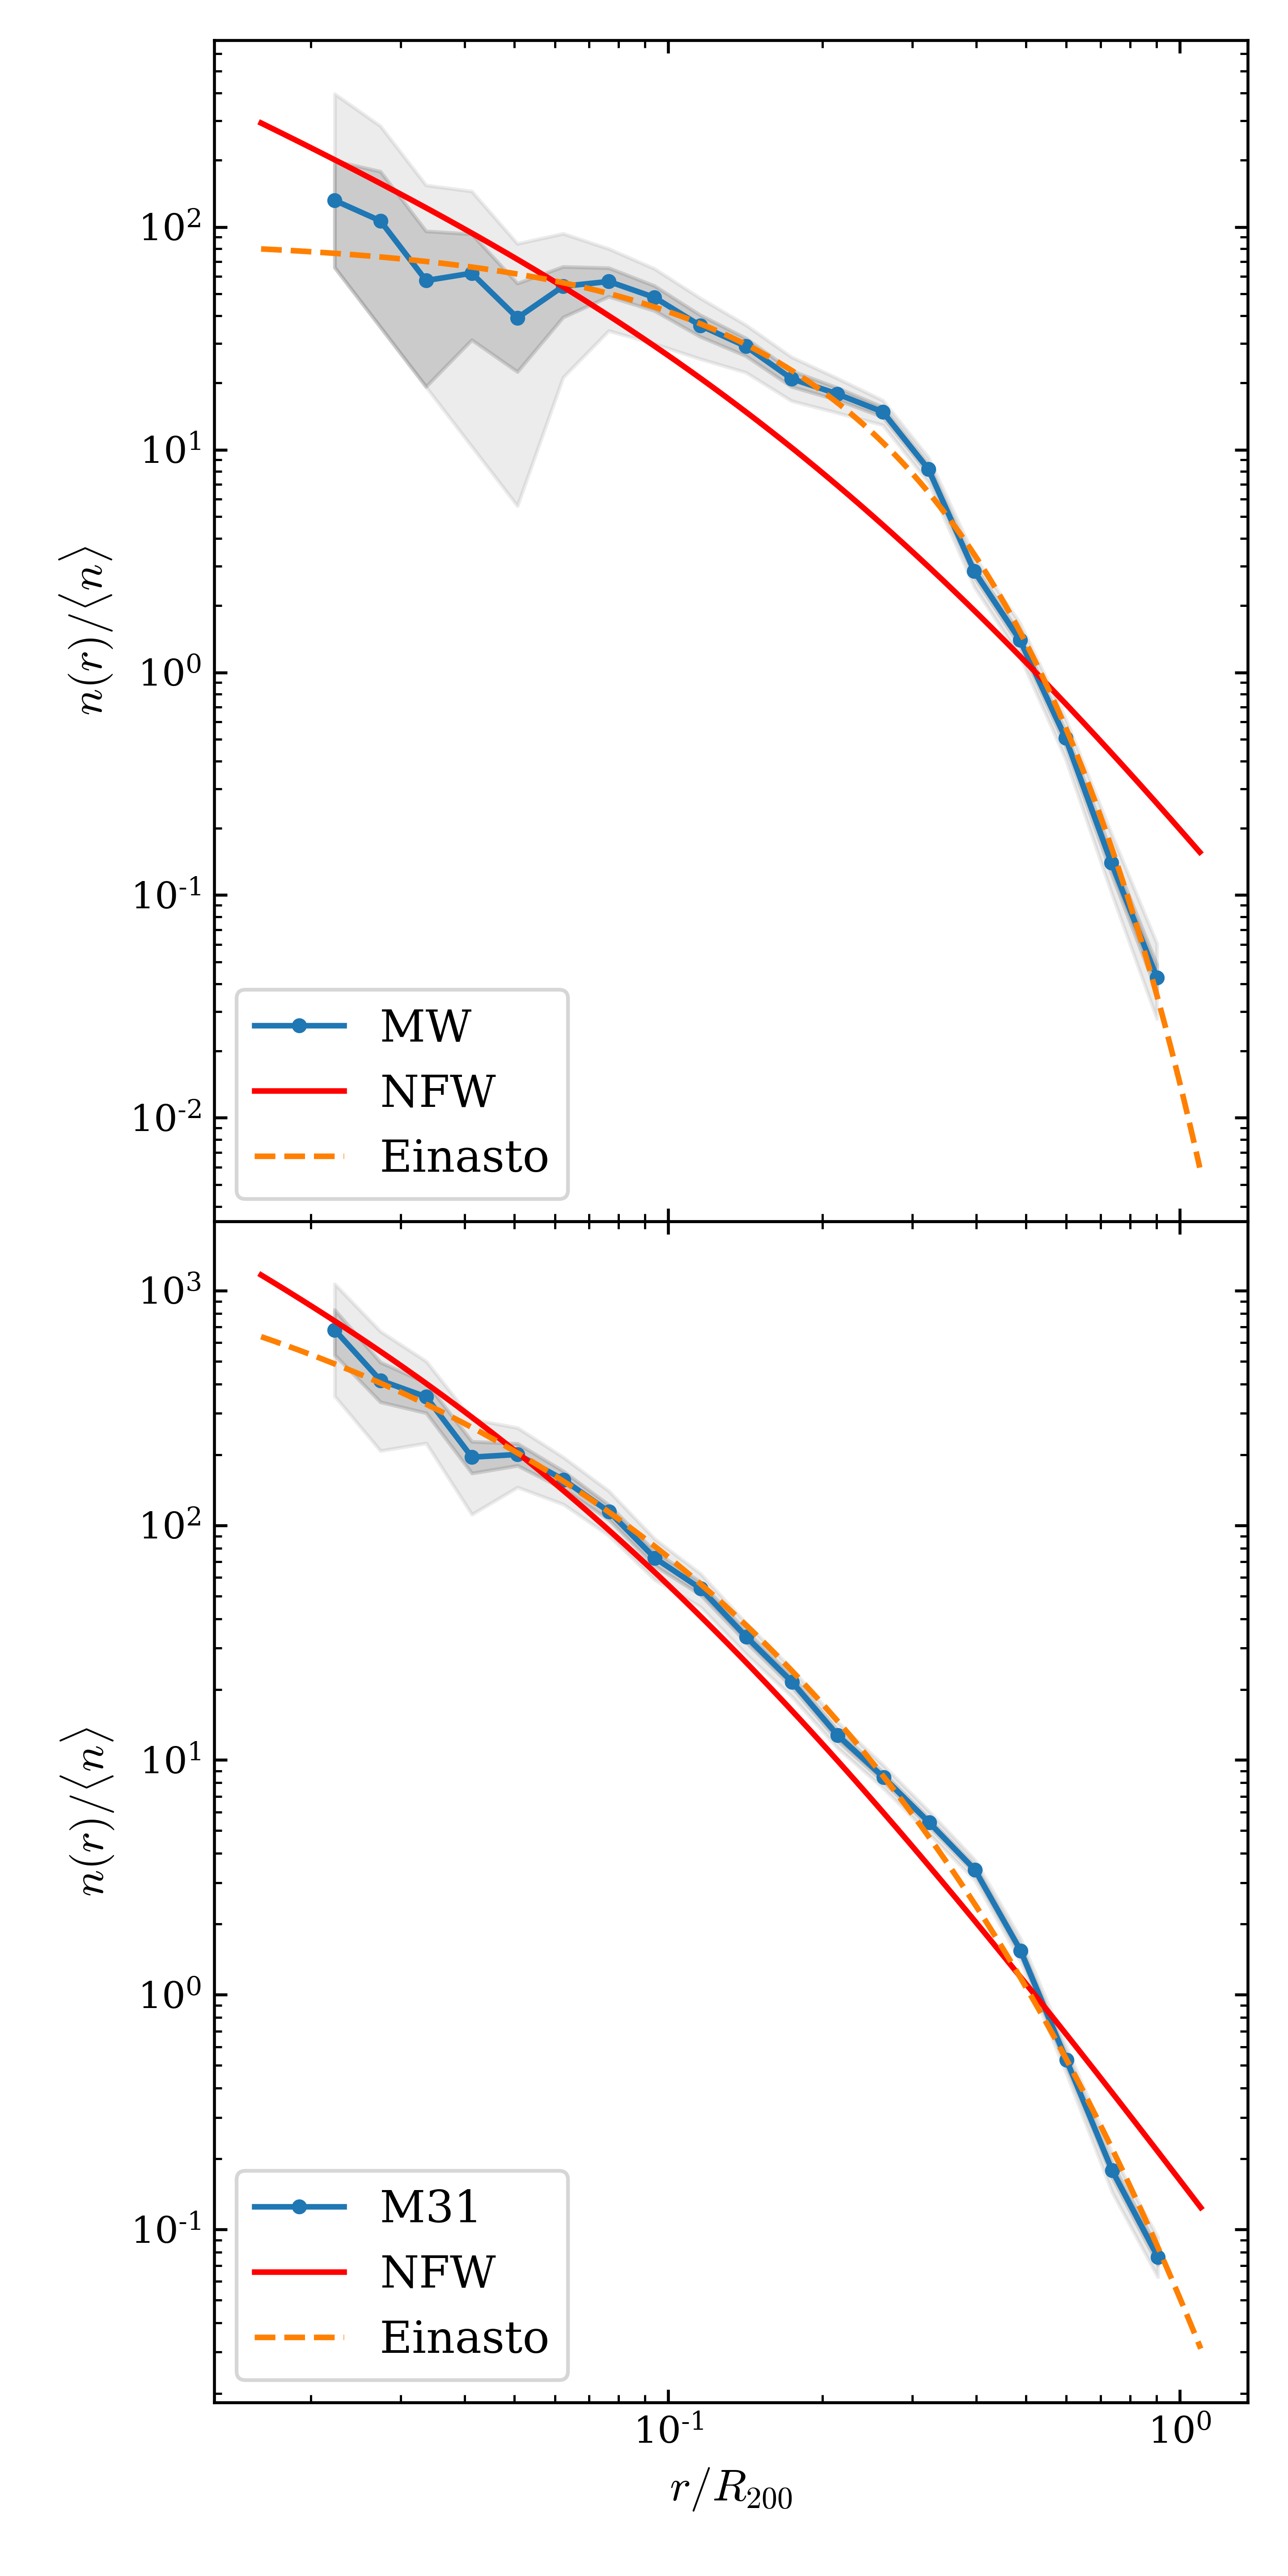
\includegraphics[width=0.5\textwidth]{20180316_121626_n_DENSITY_M31_FIG_20_Gyrs}
\caption{The normalised radial number density profiles for the MW (top) and M31 (bottom). The median number density profiles of the MW and M31 cores are shown with a solid line. The $1\sigma$ and $3\sigma$ confidence levels are shown as the shaded regions. NFW (solid) and Einasto (dashed) profiles have been fitted using parameters displayed in Table \ref{table: NFW/Ein params}.}
\label{fig: n density MW}
\end{figure}

Figure \ref{fig: n density MW} shows the number density profiles for the reformed galactic cores post-collision, with the fitting parameters used for the profile fits given in Table \ref{table: NFW/Ein params}. The $\chi^2_{min}$ values in Table \ref{table: NFW/Ein params} show that the Einasto profile is a much closer fit to the data than the NFW profile which is possible due to to the Einasto profile's extra free parameter, $\alpha$.

\begin{figure*}
\centering
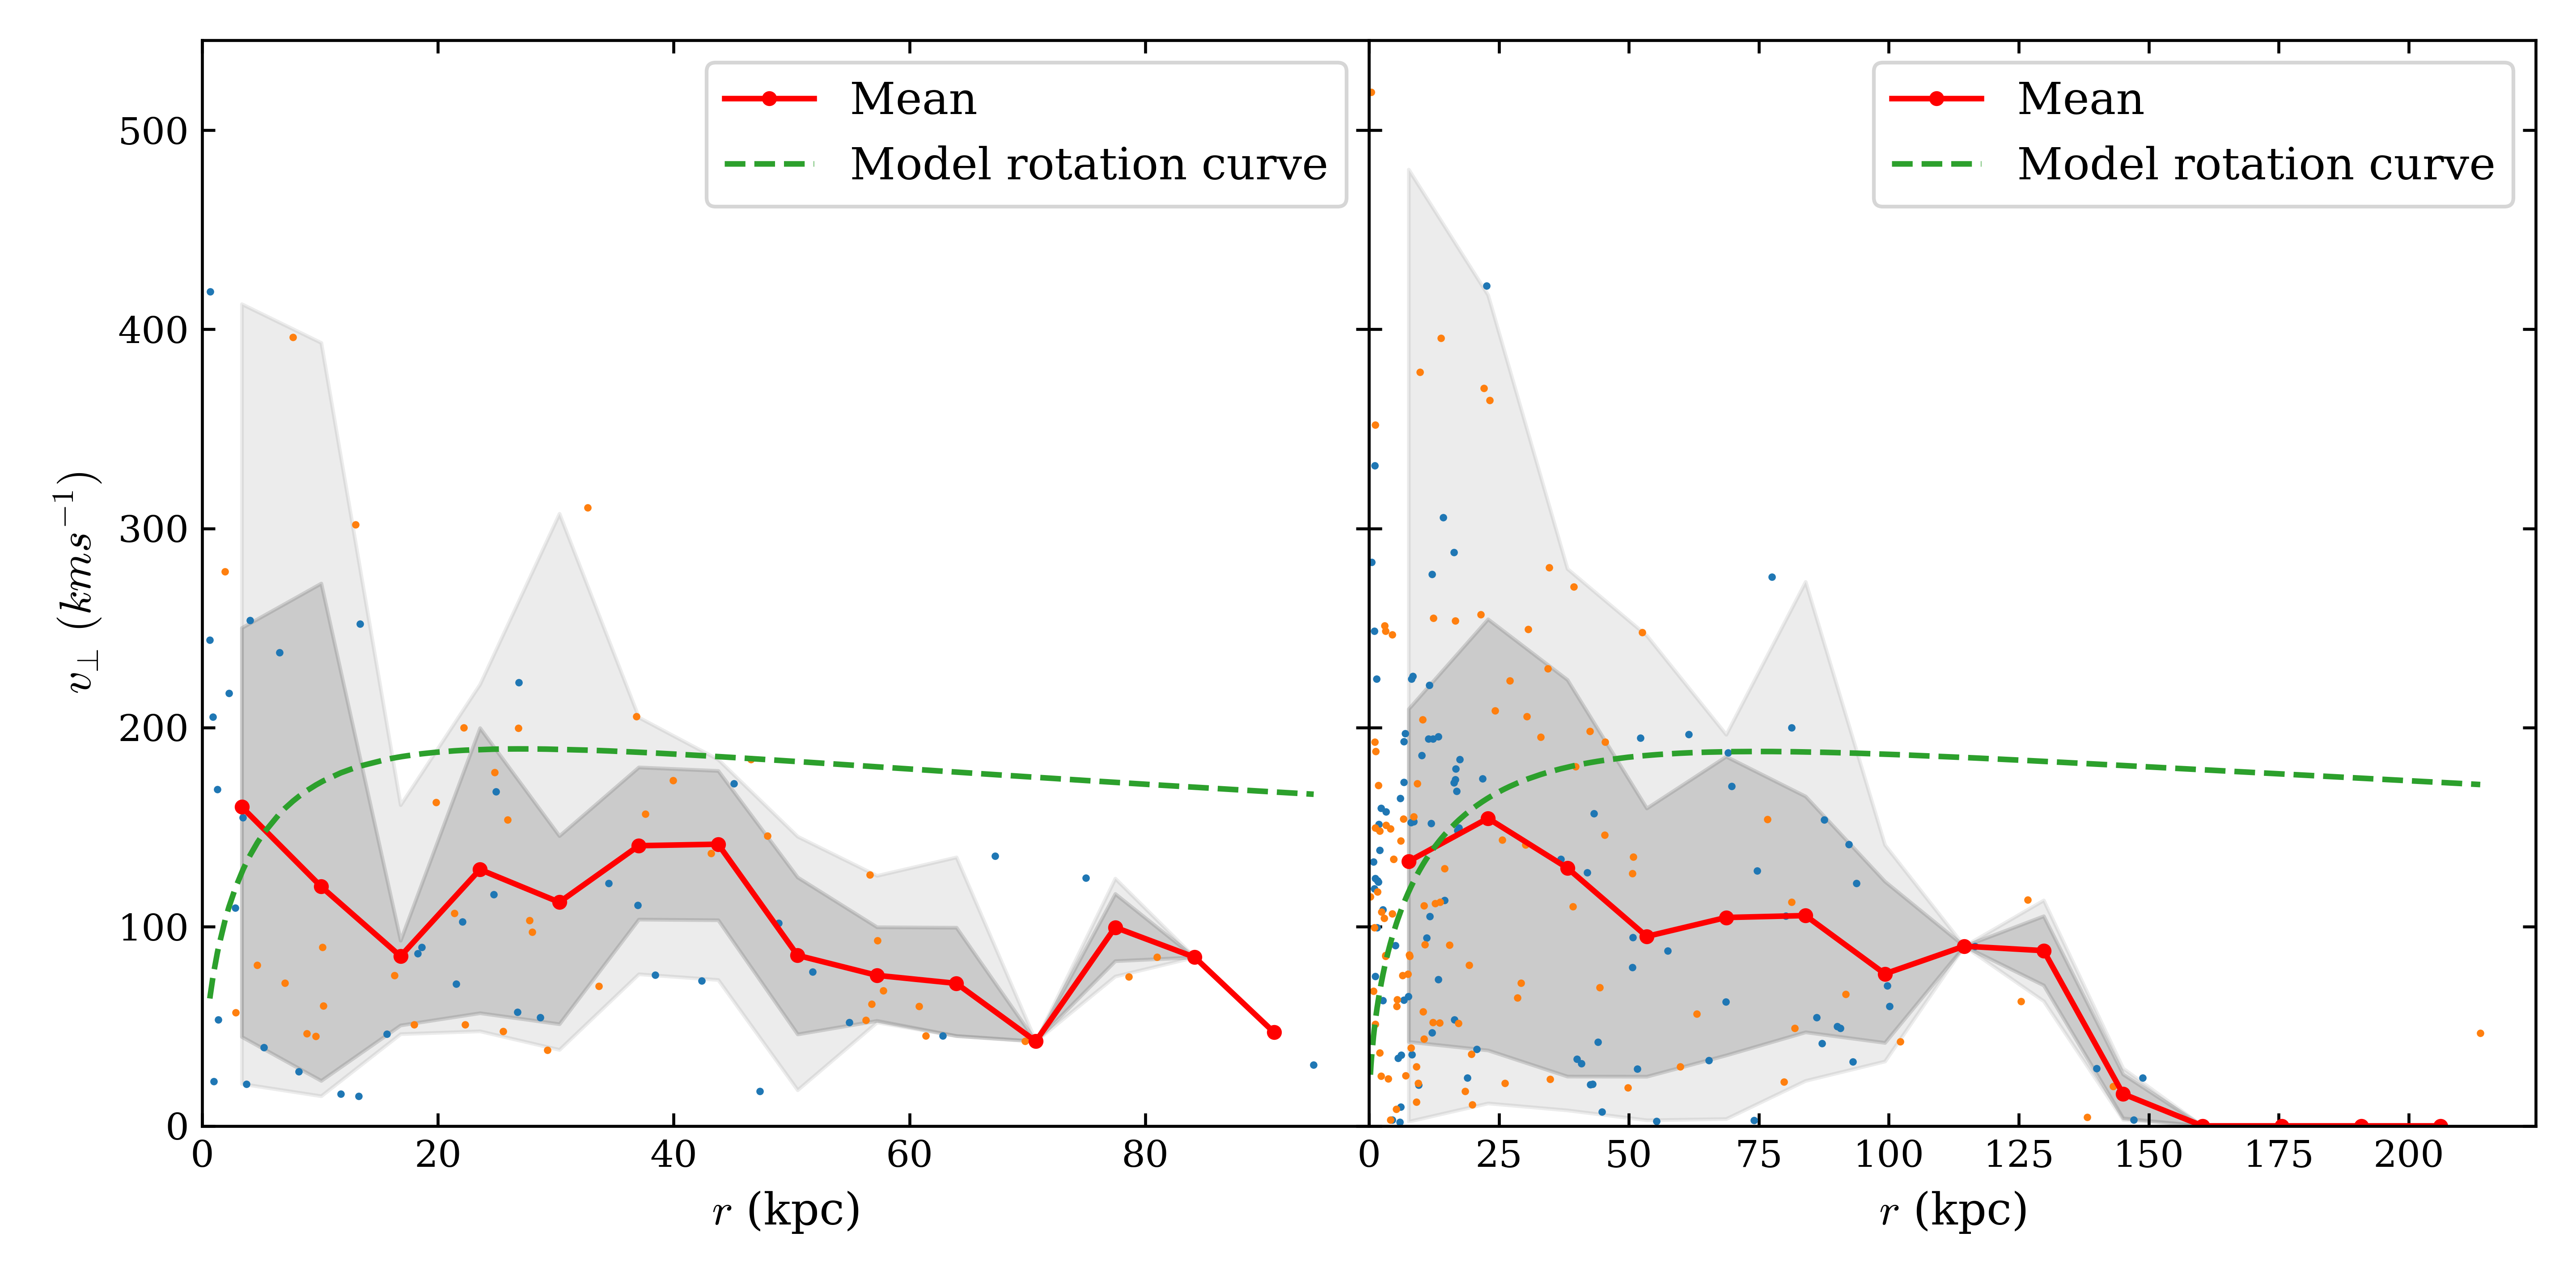
\includegraphics[width=\textwidth]{20180316_121926_ROT_CURVE_20_Gyrs}
\caption{Rotation curves for the post-collision MW (left) and M31 (right) cores. The mean rotational velocity of our binned data is given by the solid line. The raw data is given by the points with differing coloured points representing stars on opposite sides of the galactic plane. The $1\sigma$ and $3\sigma$ confidence levels are displayed as the shaded regions.}
\label{fig: ro curve MW}
\end{figure*}
%\begin{figure}[ht!]
%\centering
%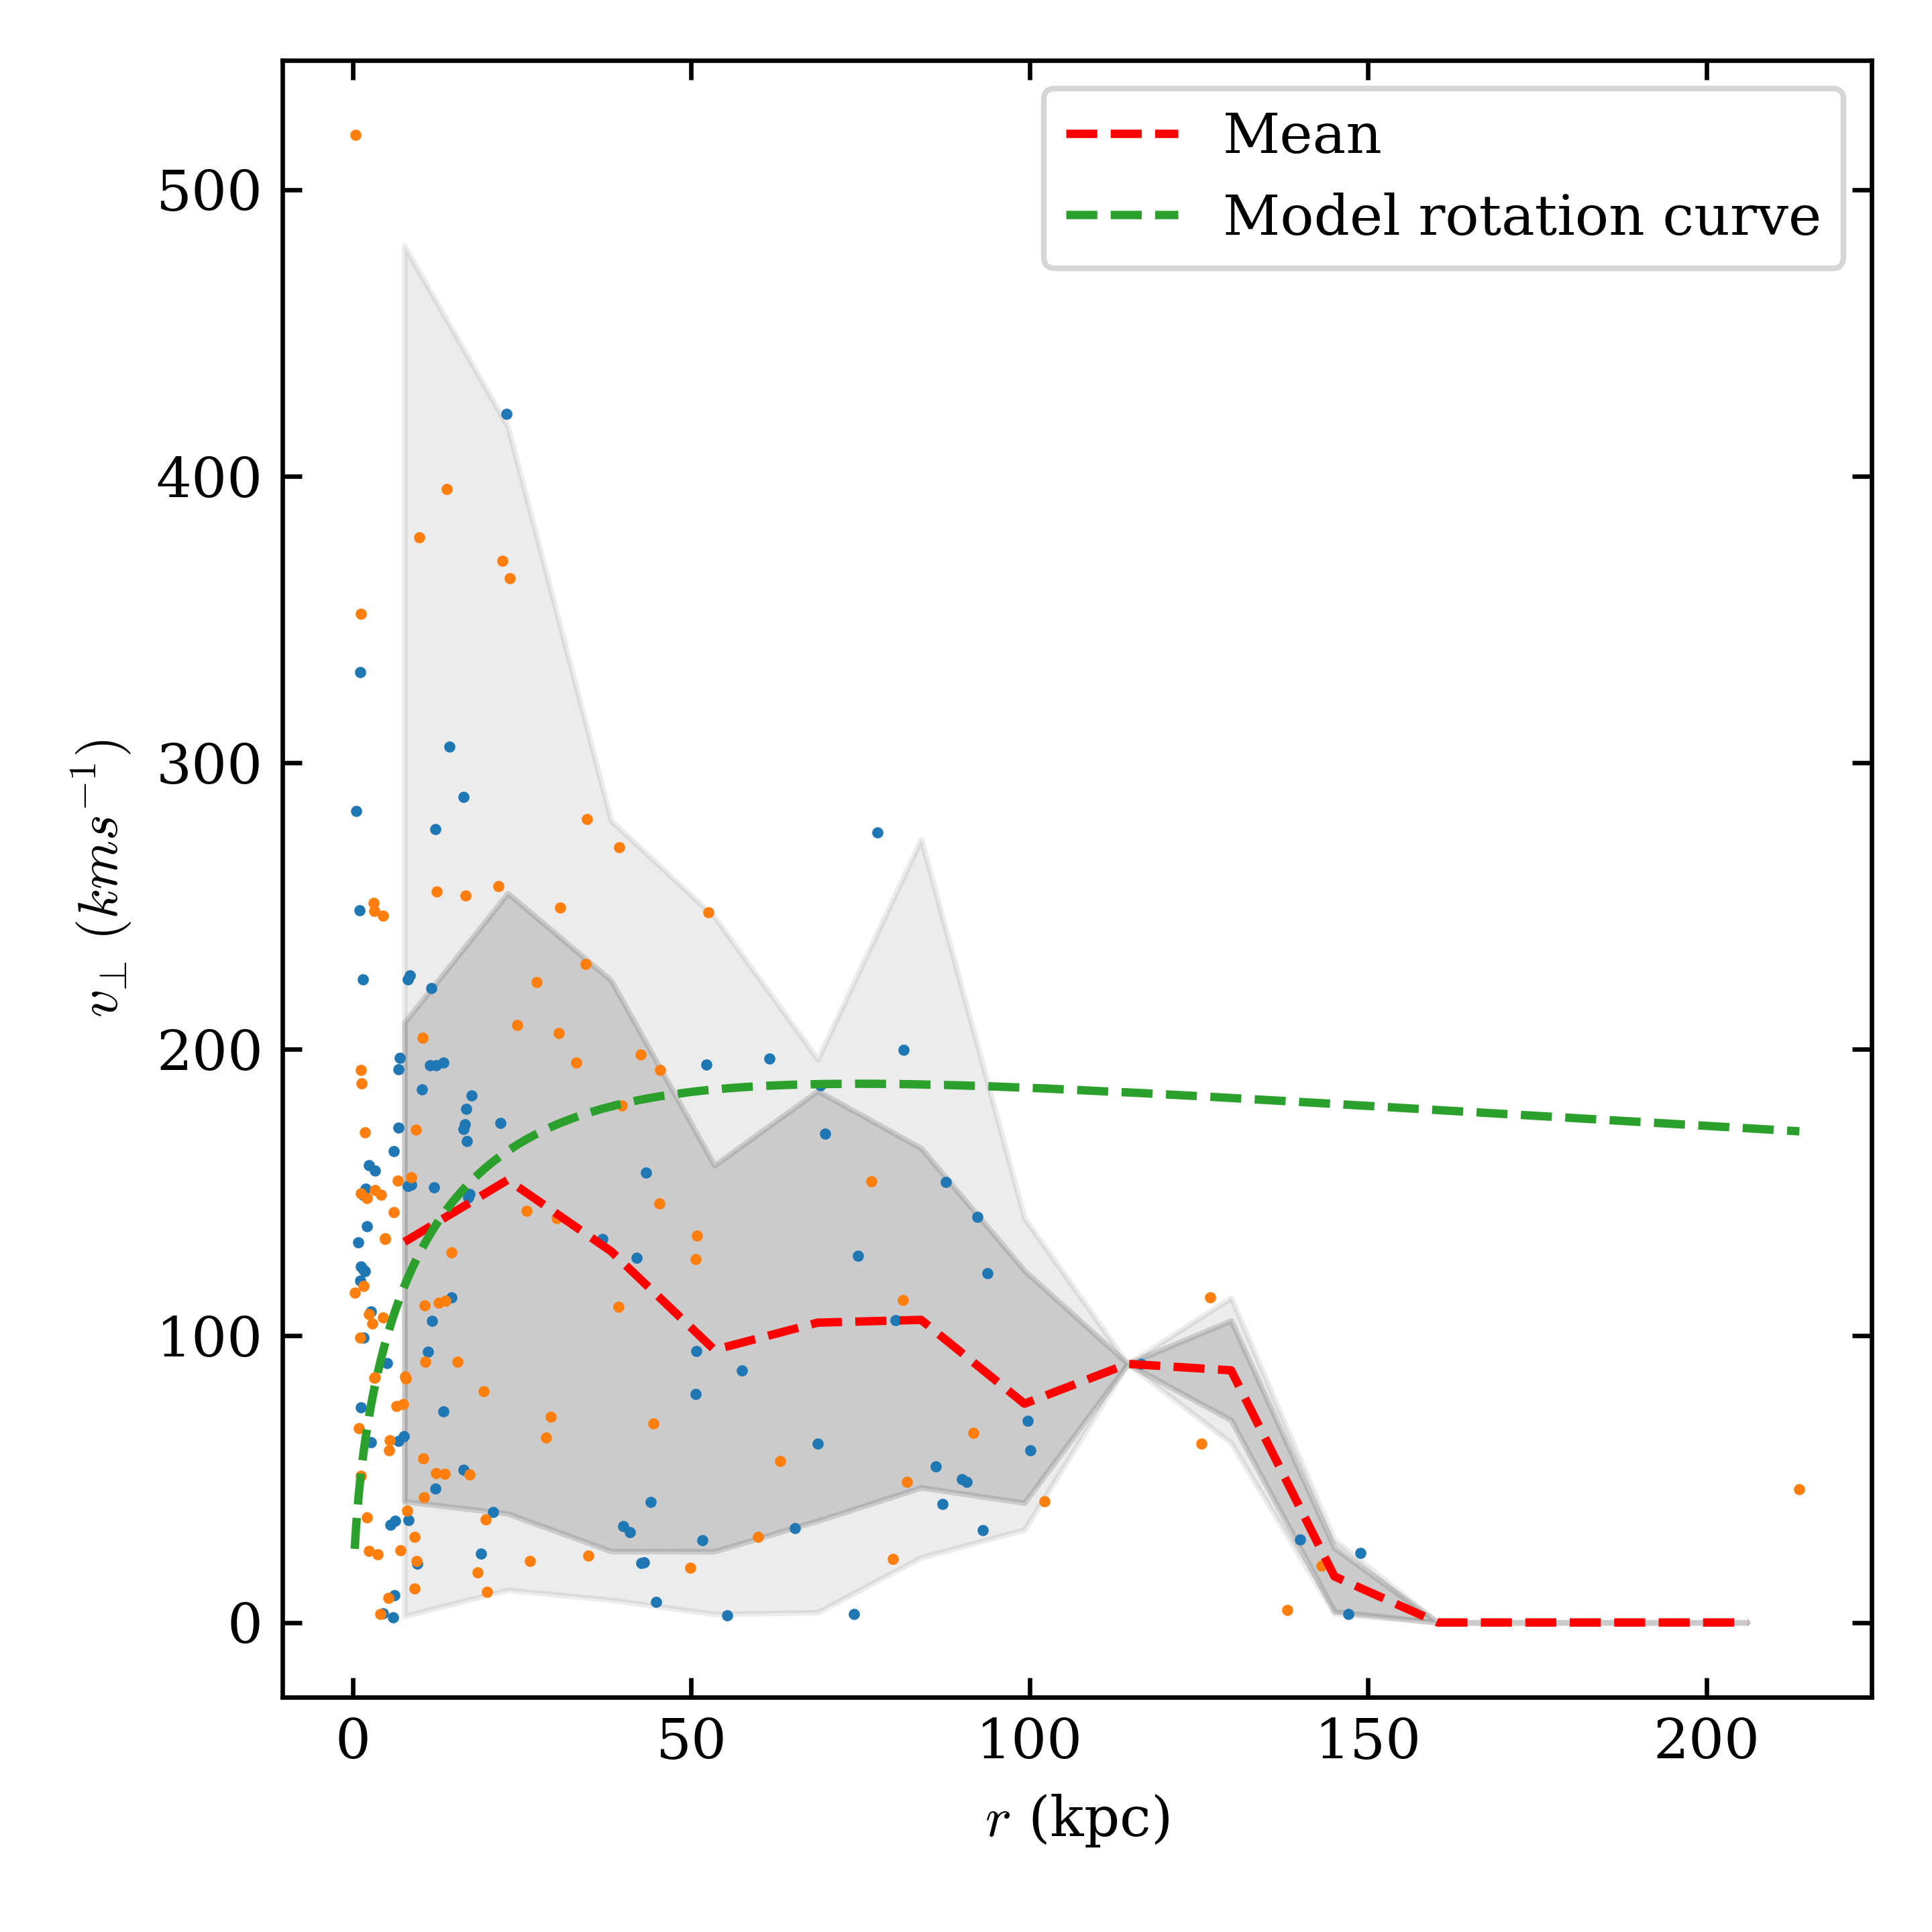
\includegraphics[width=0.5\textwidth]{20180315_014748_M31_ROT_CURVE_20_Gyrs}
%\caption{The rotation curve of our data for the M31 galactic core post-collision with $1\sigma$ and $3\sigma$ confidence levels displayed. The differing coloured data sets correspond to velocities on opposite sides of the galactic body. The red line shows the mean of binned data.}
%\label{fig: ro curve M31}
%\end{figure}
Figure \ref{fig: ro curve MW} shows the calculated perpendicular velocities of the stars in the galactic cores post-collision compared to the expected rotation curve. The mean of the data sets do not closely fit the expected model, generally lying outside the $3\sigma$ region. However, the simulation is noisy rendering the reliability of these comparisons somewhat suspect. This can be solved trivially by using more stars in the simulation.

\section{Discussion} 

The results of the integrator analysis shown in Figure \ref{fig: integrator comp} demonstrate that the Taylor method is a poor integrator for simulations where high accuracy is required, this is in agreement with the literature. We found that the Taylor method was computationally faster than the RK4 method. However, the loss in accuracy was too great a trade off as it would produce highly spurious results during the closest approach of the galaxies. At these times, the velocities of the stars and galactic cores are greatest and they move comparatively larger distances per time step than when the galaxies are further apart and moving with lower velocity.

Our softening length investigation showed that, with the parameters used in this work, the effect of $\epsilon$ on deflection angle is maximal at around $\epsilon \approx 1$ kpc as there is an inflection point here as evidenced in Figure \ref{fig: softening length comparison}. For larger values of $\epsilon$, increasing $\epsilon$ has a diminishing effect on the deflection angle of the collision. The value of $\epsilon=7.5$ kpc was selected as this gave deflection angles of $100\degree$ and $60\degree$ for MW and M31, respectively. These are more appropiate for colliding galaxies as they are lower than $180\degree$ which is the case for $\epsilon=0$. On the other hand, selecting a non-zero softening length value causes the gravitational force acting on the galactic core to behave non-clasicaclly when $r<\epsilon$. The implications of this are unknown and warrant further investigation. Different methods of modelling the galactic cores that do not involve softening could be investigated in further works as the deflection angles at $\epsilon = 7.5$ kpc are still unrealistically high for colliding galaxies. Cox and Loeb (2008) have shown that a deflection angle ${\sim}0\degree$ during the colliding galaxies first interaction is more realistic.\textsuperscript{\cite{CoxCollisionMilkyWay2008}}

The stellar retention of the resulting bodies post-collision behaved as expected; trivially the larger mass galactic core (M31) should retain a larger number of stars than its lower mass counterpart. There is a small increase in the $N_{200}/N_{inital}$ ratio during $5<t<7.5$ Gyr which is due to stellar drift soon after the collision as the stars readjust to the post-collision system. $30\%$ of the total number of stars were lost to deep space (defined as outside either galactic core's $r_{200}$ radius) due to stars interacting very closely to a galactic core's centre during the collision where the force from the galactic cores tends to infinity due to the $F\propto 1/r^2$ nature of gravity. Although some loss would be expected, this is clearly unphysical and represents a limitation of our model.

The resulting number densities of the post-collision galactic cores are shown to be better fitted by Einasto profiles than NFW profiles as shown in Figure \ref{fig: n density MW}. This is also supported by the $\chi^2_{min}$ values calculated in Table \ref{table: NFW/Ein params} with NFW producing $\chi^2_{min,MW}=18.17$ and $\chi^2_{min,M31}=9.97$, whereas Einasto produces $\chi^2_{min,MW}=0.66$ and $\chi^2_{min,M31}=1.38$. The literature documents that dark matter halos are well fitted by both NFW and Einasto profiles; however, our work supports the areas of the literature suggesting that Einasto better fits real-world dark matter halos.\textsuperscript{\cite{AnFittingfunctionsdark2013}}
These results are significant as they show that the stars in our models can form density profiles as expected in more complex computational models performed in the literature.\textsuperscript{\cite{CoeDarkMatterHalo2010}} These results were produced using numerous simplifications to the N-body simulation and using softened point masses for the galactic cores which shows how a highly simplified model can be used to generate results that are in agreement with the predictions from the literature. The simplifications used in this model still allowed NFW and Einasto density profiles to form with a good level of fit, shown by the $\chi^2_{min}$ values in Table \ref{table: NFW/Ein params}, and so we conclude that the use of the restricted three body principle would be viable to analyse number density profiles if N-body simulations were not possible.

The analysis of the post-collision rotation curves produced poor results that were not in agreement with the expected result. There are multiple possible reasons for this: firstly, the data set is very noisy; this would be trivially improved by more stars used in the simulation. Secondly, the lack of literature rotation curves may be a limitation of the model we have used. The dark matter halo associated with each core is fixed and so when the two dark matter halos begin to overlap due to the colliding galaxies, their interaction with each other is not properly modelled and requires a more complex evolving dark matter halo implementation. The NFW profile being modelled is only valid for virialized dark matter halos which is clearly not the case during collision. A further limitation of the model is that the stars themselves do not interact with each other. Galaxy discs form from rotating clouds of gas that condense to the principal plane of rotation through the transfer of angular momentum.\textsuperscript{\cite{EggenEvidencemotionsold1962}} As the stars in this simulation are modelled as test particles, they are not able to transfer momentum between themselves or the massive galactic cores.

We find that modelling colliding galaxies as a restricted three body system can be viable for exploring the transfer of stellar matter between galaxies and the number density profiles of the stars in the resulting post-collision bodies. However, this method cannot be used to investigate the rotation curves of these bodies due to the limitations of the model used, whereby it is not possible for the stars to interact with each other or influence the galactic cores themselves. It would require full N-body simulations to explore this process.


\section{Conclusions}
 
This investigation used the principle of the restricted three body problem to simulate colliding galaxies. We explored the viability of this method by analysing the stellar transfer, number density profiles and the rotation curves of the post-collision bodies. The galaxies were modelled as massive central cores with masses based on the Milky Way and Andromeda, with the stars modelled as test particles that could not interact with each other or influence the massive cores. The galactic cores were gravitationally softened to reduce the deflection angle of the interaction and to produce an interaction in greater agreement with the literature.

We investigated the accuracy of the Taylor, RK4 and SciPy black box integrators and found that RK4 and SciPy were very similar in their accuracies but Taylor was very poor in comparison, producing a chaotic solution. The effect of varying the softening length on the deflection angle in the collision was investigated and an optimal softening length of $\epsilon=7.5$ kpc was selected.

The galaxies were simulated for 20 Gyrs using a time step of $2 \times 10^5$ years as this allowed enough time for the colliding galaxies to reform two distinct bodies. The stellar transfer analysis produced results showing that the M31 core retained a much larger fraction of stars during the collision with $N_{200}/N_{initial}\approx 1$ whereas the MW core lost $60\%$ of its stellar complement. $30\%$ of the total initial stars were lost and outside either core's $r_{200}$ radius. The analysis of the number density profiles showed that the Einasto profile with fitting parameters $\alpha=1.07^{+0.08}_{-0.09}$, $r_{-2}=47^{+3}_{-3}$,  $r_{200}=196^{+1}_{-1}$ for the MW core and $\alpha=0.47^{+0.02}_{-0.03}$, $r_{-2}=32^{+2}_{-1}$,  $r_{200}=237^{+1}_{-1}$ for the M31 core produced a good fit to our data, with $\chi^2_{min,MW}=0.66$ and $\chi^2_{min,M31}=1.38$. The rotation curves that were measured did not match the expected rotation curve. This could be due to using an insufficient number of test particles, poor modelling of the dark matter halo or the lack of interacting star particles.

Our results show that this model is viable to analyse the stellar transfer or number densities of the resulting post-collision bodies, as it produces density curves that are well fit by models in the literature. However, it is not possible to use this method to analyse the rotation curves of these bodies as this relies on inter-particle interactions. In this case a full N-body simulation would be required.

\vspace{1ex}
%\begin{acknowledgments}
%(OPTIONAL) The author would like to thank...
%
%\end{acknowledgments}
%
%
%\begin{thebibliography}{}
\normalem
\bibliographystyle{ieeetr}
\bibliography{Bibliography}
%
%
%\bibitem{ref01} A. N. Other, Title of the Book, edition, publishers, place of publication (year of publication), p. 123.   % example reference 


%\end{thebibliography} 


\end{document}